% !TEX root = B99_main.tex



The proposed framework is shown schematically in Figure \ref{fig:workflow2}. In brief, it consists of five stages. First, the radiation on the PV panels and office window is calculated for a single configuration of the ASF. The radiation results on the PV panels are then used to calculate the electricity generation. The radiation results on the window are imported into a building thermal model, and a separate lighting model. Finally, an exhaustive search of all possible configurations is performed to determine the optimal configuration for maximum energetic performance. The framework along with installation guides are publicly available for download \cite{ASFGitHub,RCGitHub} . The following subsections detail these five stages.



\begin{figure}
\begin{center}
\begin{tikzpicture}[node distance = 2cm, auto]
    % Place nodes
    \node [block] (m1) {Initialisation};
    \node [block, below of=m1, node distance=4cm] (init) {Radiation Analysis};
    \node [block, below left of=init, node distance=4cm] (circuit) {PV Circuit Simulation};
    \node [block, below of=init, node distance=2.83cm] (rc) {RC Model};
    \node [block, below right of=init, node distance=4cm] (light) {Daylighting Model};
    \node [block, below right of=circuit, node distance=4cm] (optimise) {Optimisation};
    \node [text width = 5cm, below of=optimise] (result) {Optimal Configuration and Energy Performance for $t_k$};

    % Draw edges
    \path [line] (m1) -- node[ text width=3.2cm, auto, xshift=0em] {-Facade Geometry \\ -Weather Data \\ -Building Data \\ -Orientation}(init);
    \path [line] (optimise) -- (result);
    \path [line] (init) -- (circuit);
    \path [line] (init) -- (rc);
    \path [line] (init) -- (light);
    \path [line] (circuit) |- node[near start, text width=2cm, left, yshift=0.7em] {Electricity \\ Supply} (optimise);
    \path [line] (rc) -- node[anchor=center, text width=3cm, right, xshift=0em] {Heating/ \\ Cooling \\ Demand} (optimise);
    \path [line] (light) |- node[near start, text width=3cm, right, yshift=0.8em] {Lighting \\ Demand} (optimise);
    \path [line, dashed] (result) -- ++(6cm,+0cm) |- node[near end, yshift=1.5em] {Building Data from $t_{k-1}$} (init);

\end{tikzpicture}
\caption{Simulation workflow}
\label{fig:workflow2}
\end{center}
\end{figure}



\subsection{Radiation Analysis}
\label{ch:rad}
A solar radiation simulation is run within the Rhino/Grasshopper environment \cite{grasshopper} with the Ladybug plugin \cite{roudsari2013ladybug},  that uses Radiance \cite{ward1994radiance} to determine the incident insolation on the solar facade. The solar radiation analysis implemented in Ladybug is based on the cumulative sky approach \cite{robinson2004irradiation} using the Perez All-Weather sky model and weather files with hourly resolution \cite{perez1993all}. In this analysis, the sky is divided using the Tregenza scheme \cite{tregenza1987subdivision}. The approach enables us to calculate solar irradiance on the modules, and the glazed surface behind the facade. Self shading of the PV modules is inevitable as the gap between modules is only 100mm. The modules were therefore divided with a gird size of 25mm to include the effect of mutual shading as seen in Figure \ref{fig:radiation2}.
  

\subsection{PV Circuit Simulation}

The radiation results are coupled using Python to an electrical circuit simulation of monolithically interconnected, thin-film CIGS PV modules with sub-cell level representation \cite{hofer2016parametric,python}. This model uses the standard equivalent circuit model to calculate sub-cell current-voltage curves with a single diode, one series resistor, and one shunt resistor \cite{mermoud2010}. By doing so, the electrical losses through module self shading, as described in Section \ref{ch:rad}, can be taken into account. In addition to the irradiation dependency, the PV simulation includes temperature dependency. A linear relation between PV cell operating temperature and incident solar irradiance is assumed \cite{skoplaki2009operating}. Infra-red thermal imaging at different irradiance levels was used to infer the correlation factor. Electro-thermal effects and the influence of wind are neglected in the model. For more information, please refer to the publication by Hofer et al. \cite{hofer2016parametric}.


\begin{figure}
\begin{center}
\includegraphics[width=\columnwidth, trim= 0cm 0cm 0cm 0cm,clip]{radiationAnalysis.png}
\caption{A simulation result showing module and window insolation from 11:00 - 12:00 on the 16 June for a Zurich weather file and a specific module orientation.}
\label{fig:radiation2}
\end{center}
\end{figure}


\subsection{RC Model for Building Energy Demand}

This subsection describes the formulation of a physics-based model to simulate the thermal behaviour of the building using a resistor-capacitor (RC) model. This is based on an electrical analogy corresponding to the equivalent thermal physics \cite{bacher2011identifying, sonderegger2010diagnostic, madsen1995estimation}. The model, shown in Figure \ref{fig:RC_Model}, consists of one internal thermal capacitance, and five thermal resistances. This is also known as a 5R1C model and is based on the ISO 13790 standard \cite{de2008iso}. It is briefly reviewed here for completeness.

\begin{figure}
\begin{center}
    \begin{circuitikz}
      \draw (0,0)
      node[label={left:$T_e$}] {}
      to[short,*-] (1,0)
      to[short] (1,1)
      to[european resistor=$H_w$] (3,1); % The resistor

      \draw(1,0)
      to[short] (1,-1)
      to[european resistor=$H_{em}$] (3,-1)
      node[label={10:$T_m$}] {}
      to[european resistor,l_=$H_{ms}$] (3,1)
      node[label={10:$T_s$}] {}
      to[european resistor,l_=$H_{is}$] (3,3)
      node[label={10:$T_{air}$}] {}
      to[european resistor,l_=$H_{ve}$] (1,3)
      to[short,-*] (0,3)
      node[label={left:$T_{sup}$}] {};

      \draw(3,-1)
      to[short,*-] (5,-1)
      to[short,-*] (5,1)
      to[short,-*] (3,1);

      \draw(5,1)
      to[short] (5,3)
      to[short,-*] (3,3)
      to[european current source,l_=$\phi_{HC}$] (3,5);

      \draw(5,1)
      to[european current source,l_=$\phi_{sol}+\phi_{int}$] (7,1);

      \draw(3,-1)
      to[C=$C_m$] (3,-2)
      node[ground]{};


    \end{circuitikz}
    \caption{A 5R1C Model of the single zone office space}
\label{fig:RC_Model}
\end{center}
\end{figure}


The only surface in contact with the external environment is the south facing glazed surface. All other surfaces of the room are in contact with other thermal zones of the building that are assume to hold the same room temperature. They can therefore be modelled as adiabatic surfaces. Denoting by $T_m$, the temperature of the thermal mass in the room, the differential equation for the circuit in Figure \ref{fig:RC_Model} is given by 

%Equation \ref{eq:derrive} details the equation related to the circuit in Figure \ref{fig:RC_Model} where $T_m$ is the temperature of the room mass, and $C_m$ is the thermal capacitance of the room. 


\begin{equation} 
\label{eq:derrive}
     C_m {\frac{dT_m}{dt}} + T_m(H_{tr3}+H_{em})  = \phi_{mtot}
\end{equation}

The value $\phi_{mtot}$ represents an equivalent thermal heat flux based on the solar heat gains, internal heat gains, external air temperature and the thermal conductances of the building elements. For this analysis variations of air convection caused by the solar facade are ignored. For more information on this model, refer to the Appendix, or the source code on GitHub \cite{RCGitHub}. \\

% \begin{equation} 
% \label{eq:heatflow}
%       \phi_{mtot}= \phi_m + H_eT_e + \frac{H_{tr3}}{H_{tr2}}\Big(\phi_{st} + H_wT_e + H_{tr1}T_{sup} + \frac{H_{tr1}}{H_{ve}}(\phi_{HC} + \phi_{io})\Big)
% \end{equation}



%where $C_m$ is the thermal capacitance of the room, $T_e$ is the external air, $T_{sup}$ is the conditioned air supply. The solar heat gains $\phi_{sol}$, and internal heat gains $\phi_{int}$ are represented by three equivalent heat fluxes $\phi_{io}$, $\phi_{st}$ and $\phi_m$ which correspond to a heat exchange to the air $T_{air}$, internal room surface $T_s$, and thermal mass $T_m$ respectively. The heating and cooling heat flux is represented by $\phi_{HC}$. The five thermal conductances $H$ are represented by three equivalent conductances $H_{tr1}$, $H_{tr2}$, $H_{tr3}$. For more information on the model, refer to the Appendix. 

Equation \ref{eq:derrive} is discretised using the Crank-Nicolson method so it can be solved numerically as,

%Applying the Crank-Nicolson method \cite{crank1947practical} to Equation \ref{eq:derrive} gives us the discrete differential equation described in Equation \ref{eq:derivation}. The subscripts $k$ and $k+1$ refer to the timesteps of length $\Delta t$. 

\begin{equation} 
\label{eq:derivation}
      T_{m_{k+1}}={\frac{\phi_{mtot}+T_{m_k}\Big(\frac{C_m}{\Delta t} - 0.5(H_{tr3}+H_{em})\Big)}{\frac{C_m}{\Delta t} + 0.5(H_{tr3}+H_{em})}}
\end{equation}

where the subscripts $k$ and $k+1$ refer to the time-steps of length $\Delta t$ \cite{crank1947practical}.\\

The heating or cooling demand for each time step is determined to ensure that the temperature $T_{m_{k+1}}$ is within the set thermal set points for occupant comfort. An unrestricted heating or cooling system is assumed. This means that the heating or cooling supply will always meet the calculated demand. The thermal demand is converted to electrical energy based on an average coefficient of performance (COP) of the heating or cooling system. 

\subsection{Lighting Model}
Lighting control is based on the average luminance of the room. The luminance that passes through the solar facade, to the window, is calculated in the radiation analysis in Section \ref{ch:rad}. Using the total flux method \cite{szokolay1980handbook}, the total luminance per floor area is calculated by 

\begin{equation} 
\label{eq:lighting}
      \varphi_{flux}={\frac{E_w G M U}{A_{floor}}}
\end{equation}

where $E_w$ is the incident illuminance on the window, $G$ is the solar transmittance of the window, $M$ is the maintenance factor which takes surface dust into account, and $U$ is an empirical utilisation factor based on the room dimensions and ceiling profile. If the room luminosity is less than the set threshold for comfortable lighting, and there are occupants in the room, the lights are switched on to their maximum power. When compared against a more complex Radiance model with ambient bounces there was only a 5\% divergence in results. The total flux method was therefore chosen due to its computational speed. This method however, is only applicable for small spaces. The evaluation of a hall, or an open plan working space would require a ray tracing analysis with multiple bounces. The electrical wiring and pneumatics of the ASF are encased within a reflective double curved stainless steel pipe structure that takes 6\% of the projected area. The influence of this structure can therefore be assumed to be negligible. 

\subsection{Exhaustive Search Optimisation}

At each time step the combination that minimises the net building energy demand, i.e. the difference of building energy demand for heating, cooling, lighting against BIPV electricity generation, is found using an exhaustive search of all possible configurations. Transient elements of the results, such as the temperature of the room, and thermal control settings are then stored for the next time step. It is also possible to run this optimisation to minimise individual objectives, such as heating alone.

% \begin{figure}
% \begin{center}
% 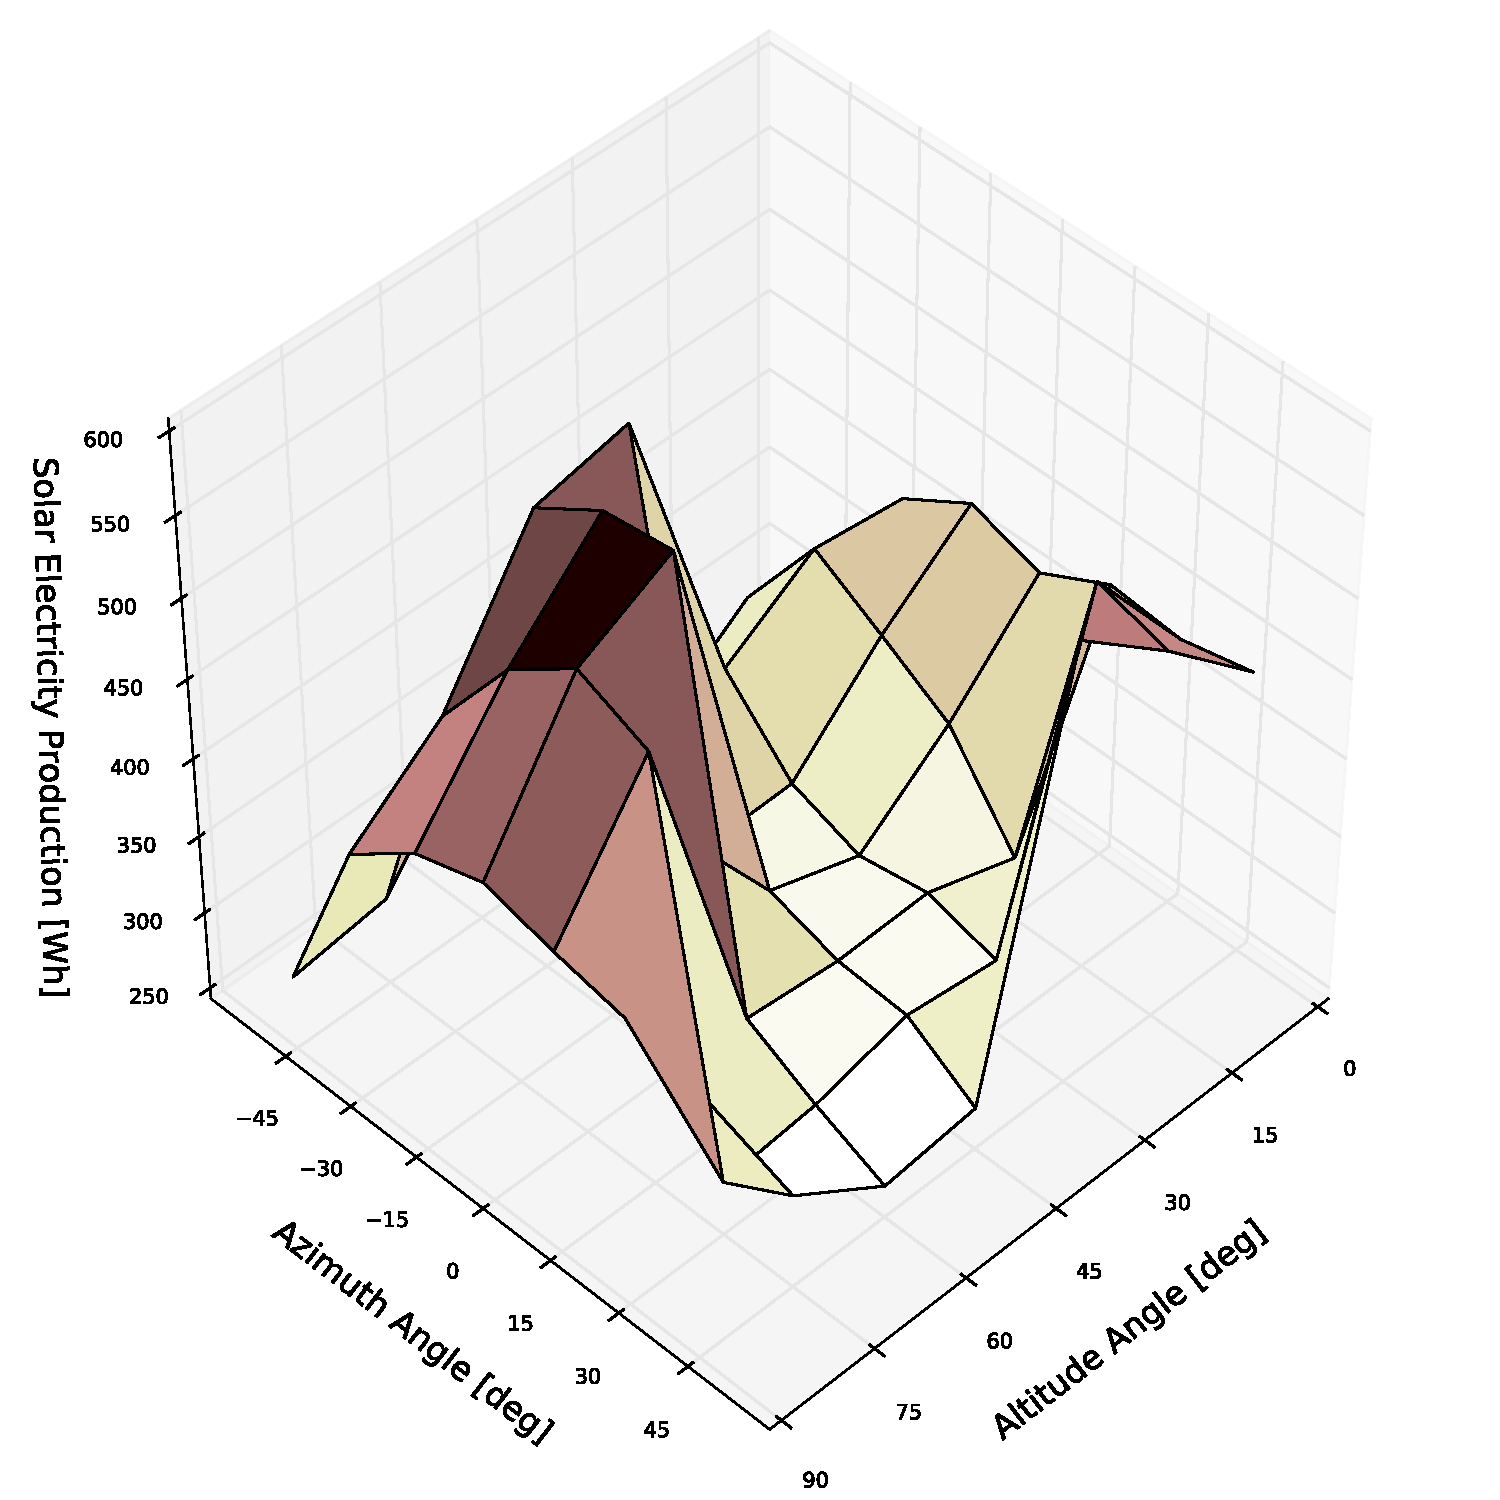
\includegraphics[width=\columnwidth, trim= 0cm 0cm 0cm 0cm,clip]{3DAnglePlot.pdf}
% \caption{ }
% \label{fig:optimsationAngles}
% \end{center}
% \end{figure}


\subsection{Case Study}

The ASF, shown in Figure \ref{fig:HoNR2}, was constructed on the House of Natural Resources at the ETH Zurich \cite{nagy2016adaptive}. This system is used as a case study for the framework. The solar facade consists of 400mm CIGS square panels that can rotate in two degrees of freedom via a soft pneumatic actuator \cite{svetozarevic2016soro}. Each panel can be independently actuated with a continuous range of actuation. However, for simplicity, all panels are grouped into one cluster that moves in unison with discrete angles. On the horizontal axis, the panels can move from 0$^{\circ}$ (closed) to 90$^{\circ}$ (open) position in steps of 15$^{\circ}$. On the vertical axis, they can move from 45$^{\circ}$ to -45$^{\circ}$ in 15$^{\circ}$ steps. This results in 49 possible dynamic configurations of the facade system.

The studied building is a two person office which is 3.1m high, 4.9m wide, and 7m deep. Input data for the simulation is based on an energy plus weather file for the Zurich region \cite{remund1997meteonorm}. The weather data is recorded at an hourly resolution, and therefore the simulation is also run at hourly time-steps. A full set of input parameters for this case study is summarised in Table \ref{tab:AssumptionsOpp}.



\begin{table*}
\centering
\begin{tabular*}{\textwidth}{ll}
\hline
\textbf{Office Zone Settings} &                                        \\
Office Envelope               & Internal Walls: Adiabatic              \\
                              & Window: Double Glazed U=1.1 $W/m^2K$     \\
                              & External Wall: U=0.2 $W/m^2K$            \\
Daylighting Variables         & Glass Solar Transmittance: 0.68                          \\
                              & Maintenance Factor: 0.9                \\
                              & Utilisation Factor: 0.7               \\
Thermal Conductances          & $H_{ve}=39 W/K  $                      \\
                              & $H_{w}=14.9 W/K $                      \\
                              & $H_{em}=0.34 W/K$                      \\
                              & $H_{is}=491 W/K $                      \\
                              & $H_{ms}=780 W/K $                      \\
Thermal Set Points            & Heating: 22$^{\circ}$C                 \\
                              & Cooling: 26$^{\circ}$C                 \\
                              & Set-Back: 4$^{\circ}$C                 \\
Building System               & Lighting Load: 11.8 $W/m^2$             \\
                              & Lighting Control Threshold: 300 lx     \\
                              & COP Heating: 3                         \\
                              & COP Cooling: 3                         \\
Occupancy                     & Office Schedule  \cite{CEAToolbox}     \\
                              & Ventilation: 1.5 air changes per hour  \\
                              & Infiltration: 0.5 air changes per hour \\
                              & Human Heat Emission: 120$W$ per person                                       \\
\textbf{Location Assumptions} &                                        \\
Weather File                  & Zurich-Kloten, Switzerland 2013 \cite{remund1997meteonorm}       \\
Window Orientation                   & South                                  \\
\hline
\end{tabular*}
\caption{Summary of simulation parameters}
\label{tab:AssumptionsOpp}
\end{table*}





